\documentclass{article}
\usepackage{geometry}
\usepackage{lipsum} 
\usepackage{listings}
\usepackage{graphicx}


\title{Initial Results and Discussion}
\author{Kuang Sheng}
\date{April 29th, 2024}

\begin{document}

\maketitle

\section*{Research Question}
What is the true value of urban green space (UGS) in the city of Chicago?

\section*{Description}
I collected property listing data from Redfin and performed a spatial analysis in a pilot study to understand the relationship between property listing price and the property’s locational and internal features. Here are some initial results and visualizations of machine learning tasks of the pilot study.

\subsection*{Workflow Presentation}
\begin{figure}[h]
  \centering
  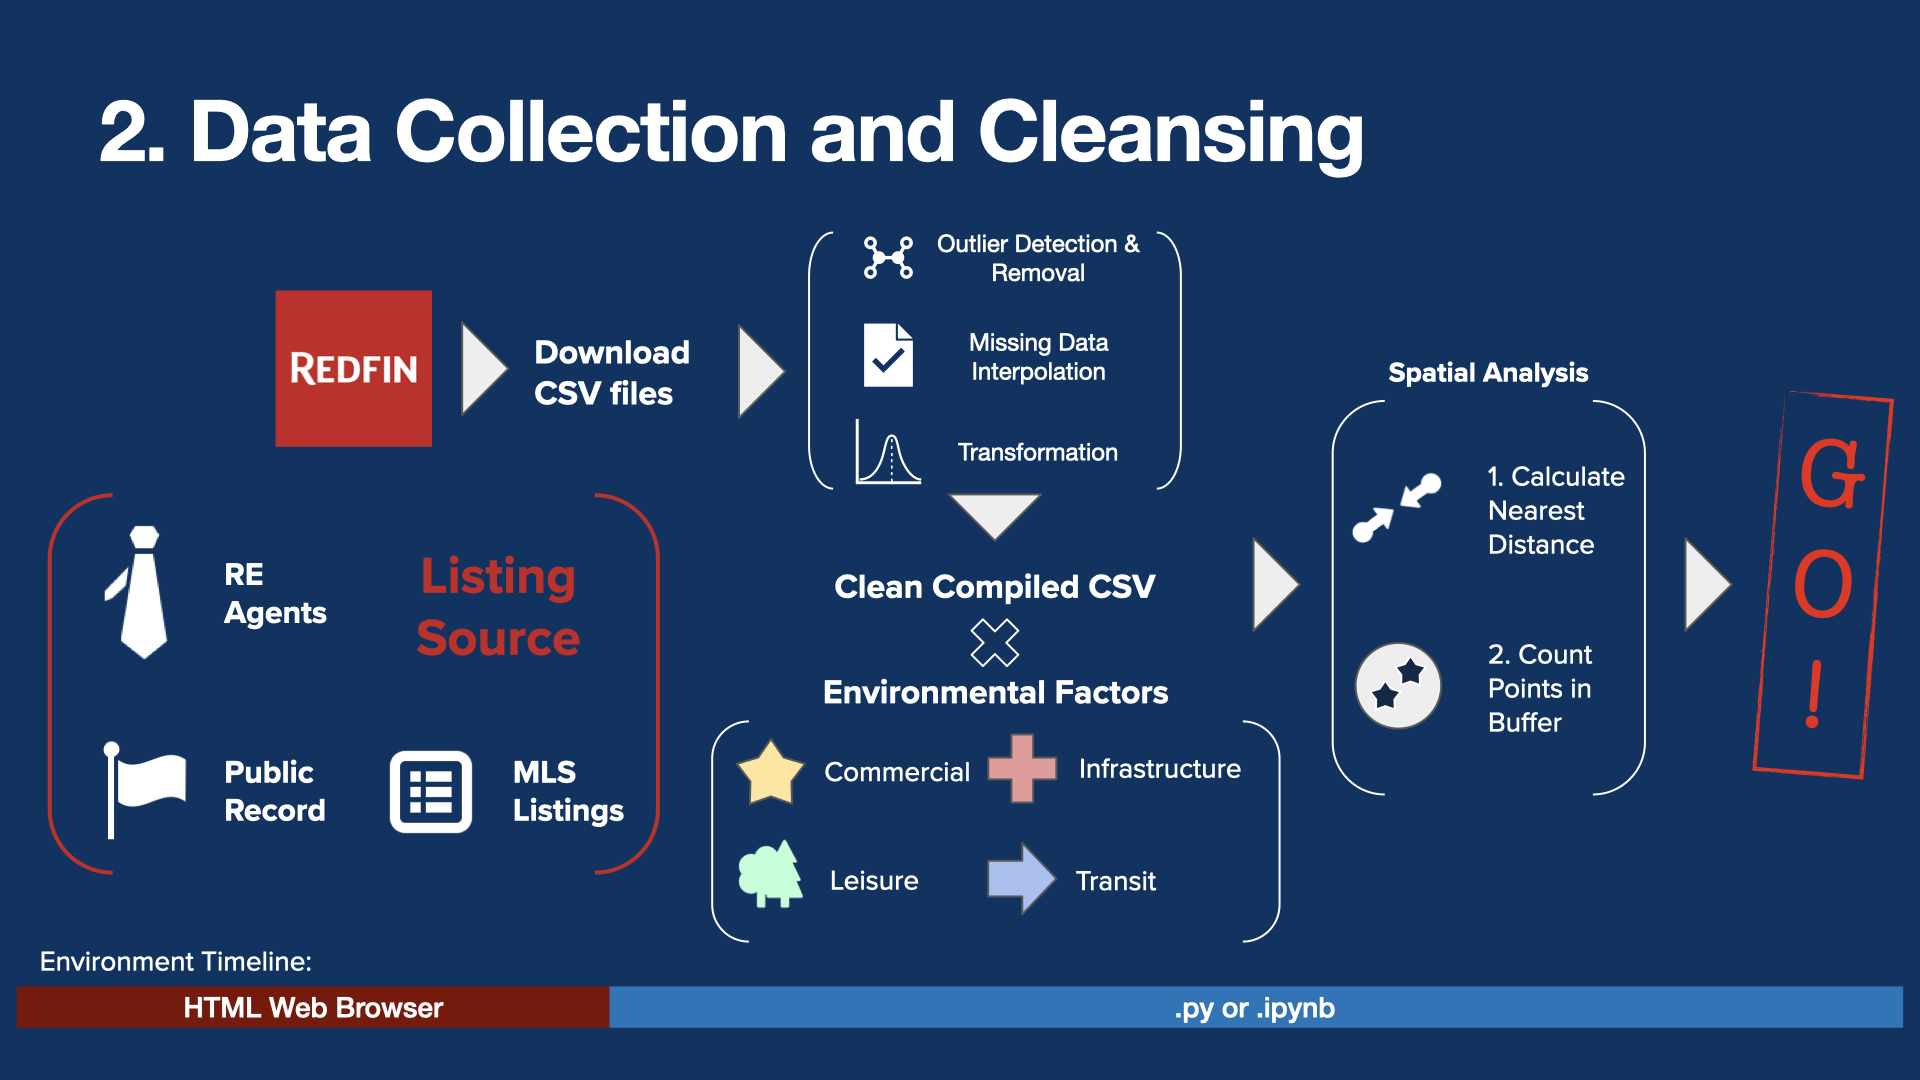
\includegraphics[width=\textwidth]{Visual/workflow.jpeg}
  \caption{Workflow Presentation}
\end{figure}

Figure 1 shows the workflow of my pilot study. For my research design, I will enrich the data complexity and accuracy at the spatial analysis stage by incorporating NDVI calculated based on the USGS satellite imagery data to compare the machine learning results.

\subsection*{Correlation Heat Map(Figure 2)}
\begin{figure}[h]
  \centering
  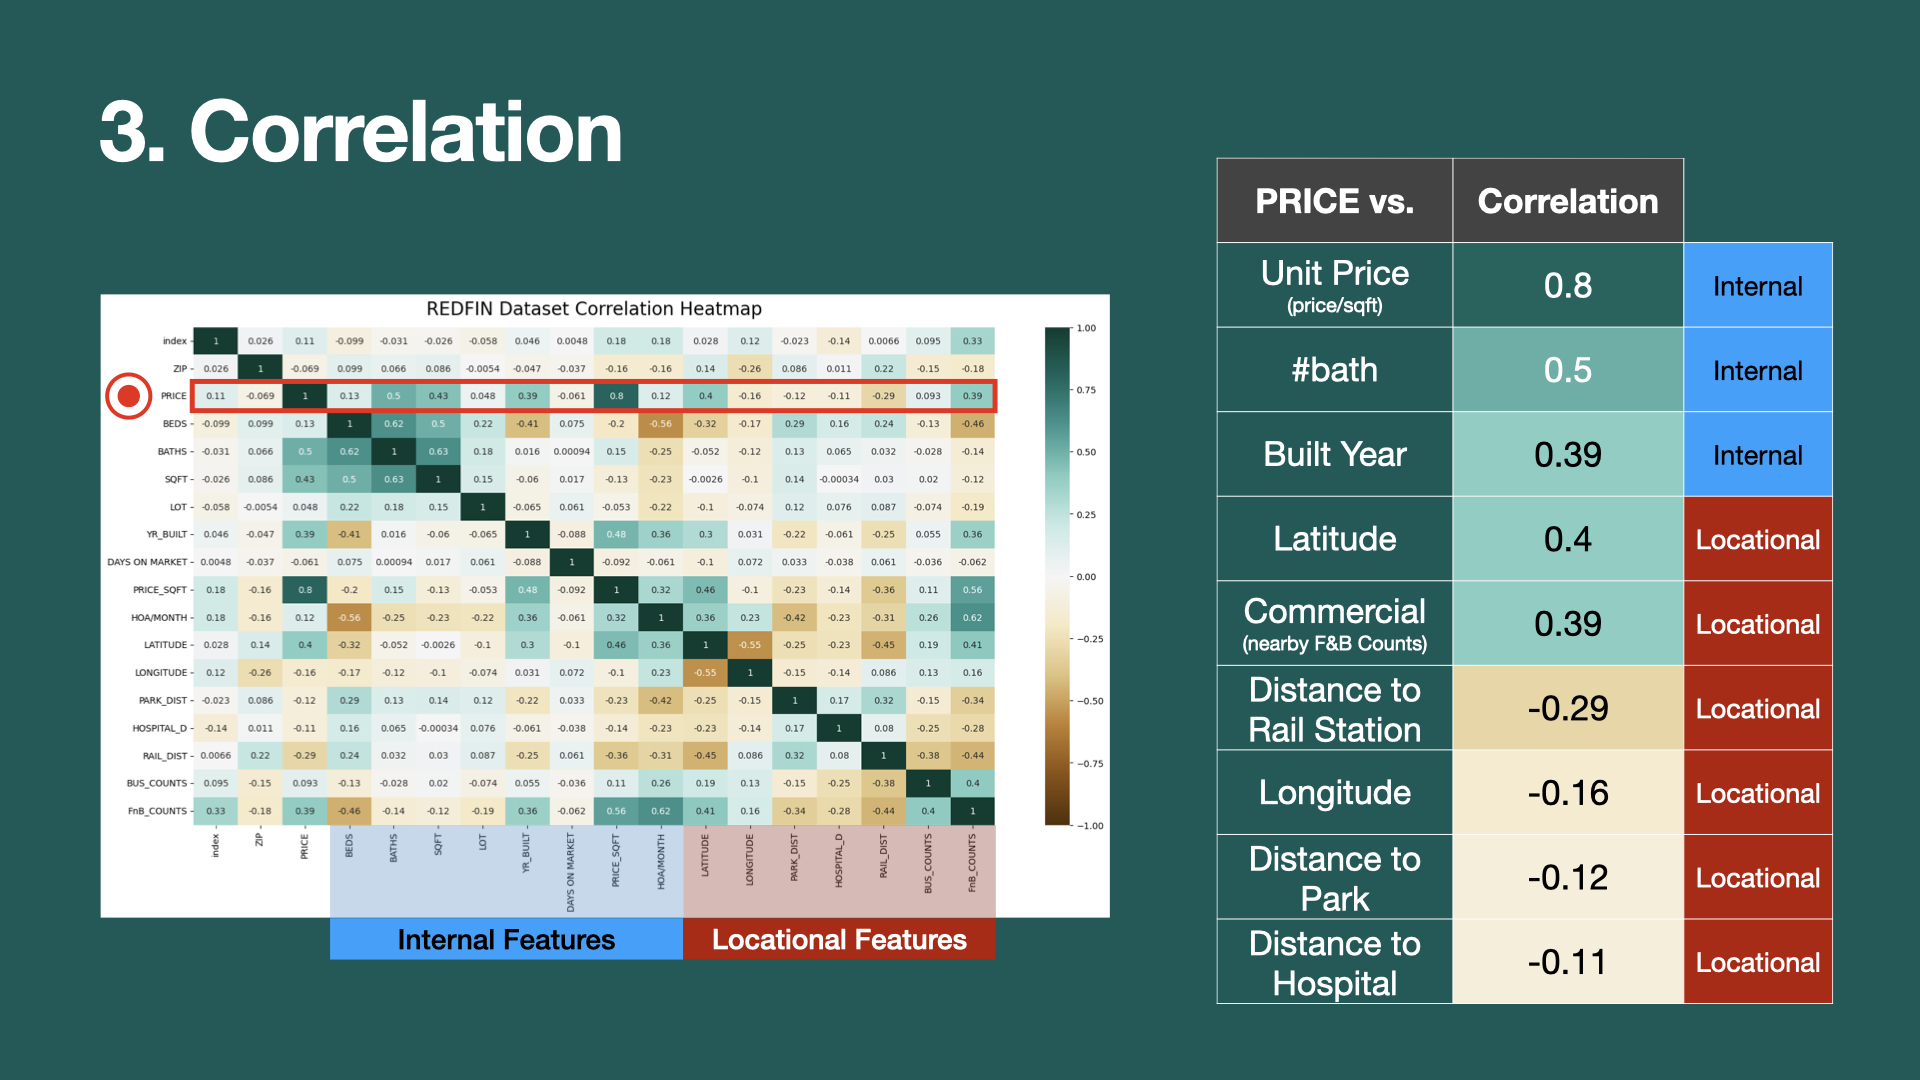
\includegraphics[width=\textwidth]{Visual/heatmap.jpeg}
  \caption{Correlation Heat Map(Figure 3)}
\end{figure}

\subsection*{Initial Results}
\begin{figure}[h]
  \centering
  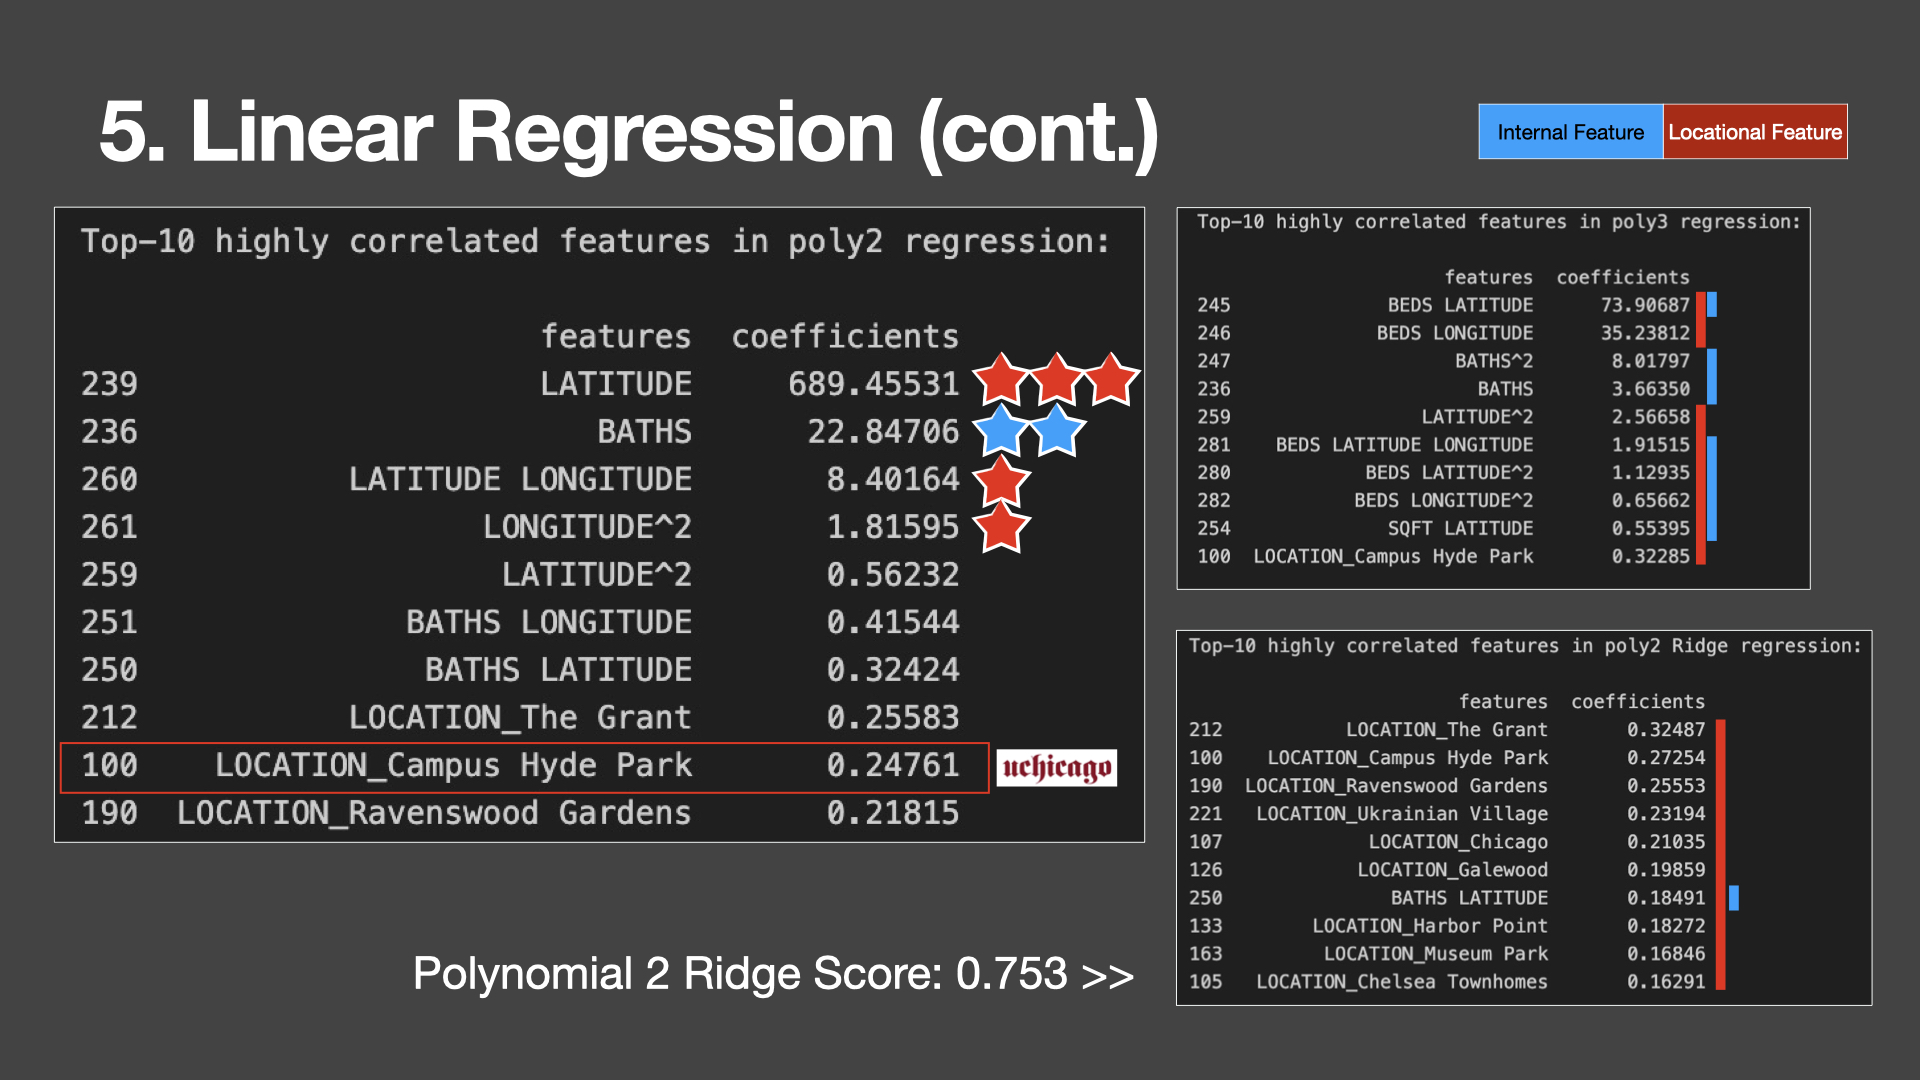
\includegraphics[width=\textwidth]{Visual/results.jpeg}
  \caption{Initial Results}
\end{figure}

In the correlation heat map, park proximity (distance to park) shows a negative correlation with the housing price, which contradicts the theories and research outcomes in the literature review. I assume this is caused by the deficiency of the current UGS dataset. In the Initial Results, the graph shows the coefficient of the different features in the optimal machine learning model. Both locational and internal features play an important role in predicting the housing price. However, locational features play a more significant role here. Unfortunately, based on the result of current park proximity data, I did not discover a significant correlation or causing factor. I plan to compare the results of the analysis that includes satellite imagery data with the current data to see if the UGS-related features become more significant with the enhanced dataset.

For mocked-up results, I plan to show the coefficient ranking based on the satellite imagery data and compare it with the pilot study to see if the data enrichment and enhancement add more weight to the predicting capabilities of UGS. Also, I plan to visualize the different features discussed using maps to better visualize the interrelation with property value.

\subsection*{Example Map(Figure 4)}
\begin{figure}[h]
  \centering
  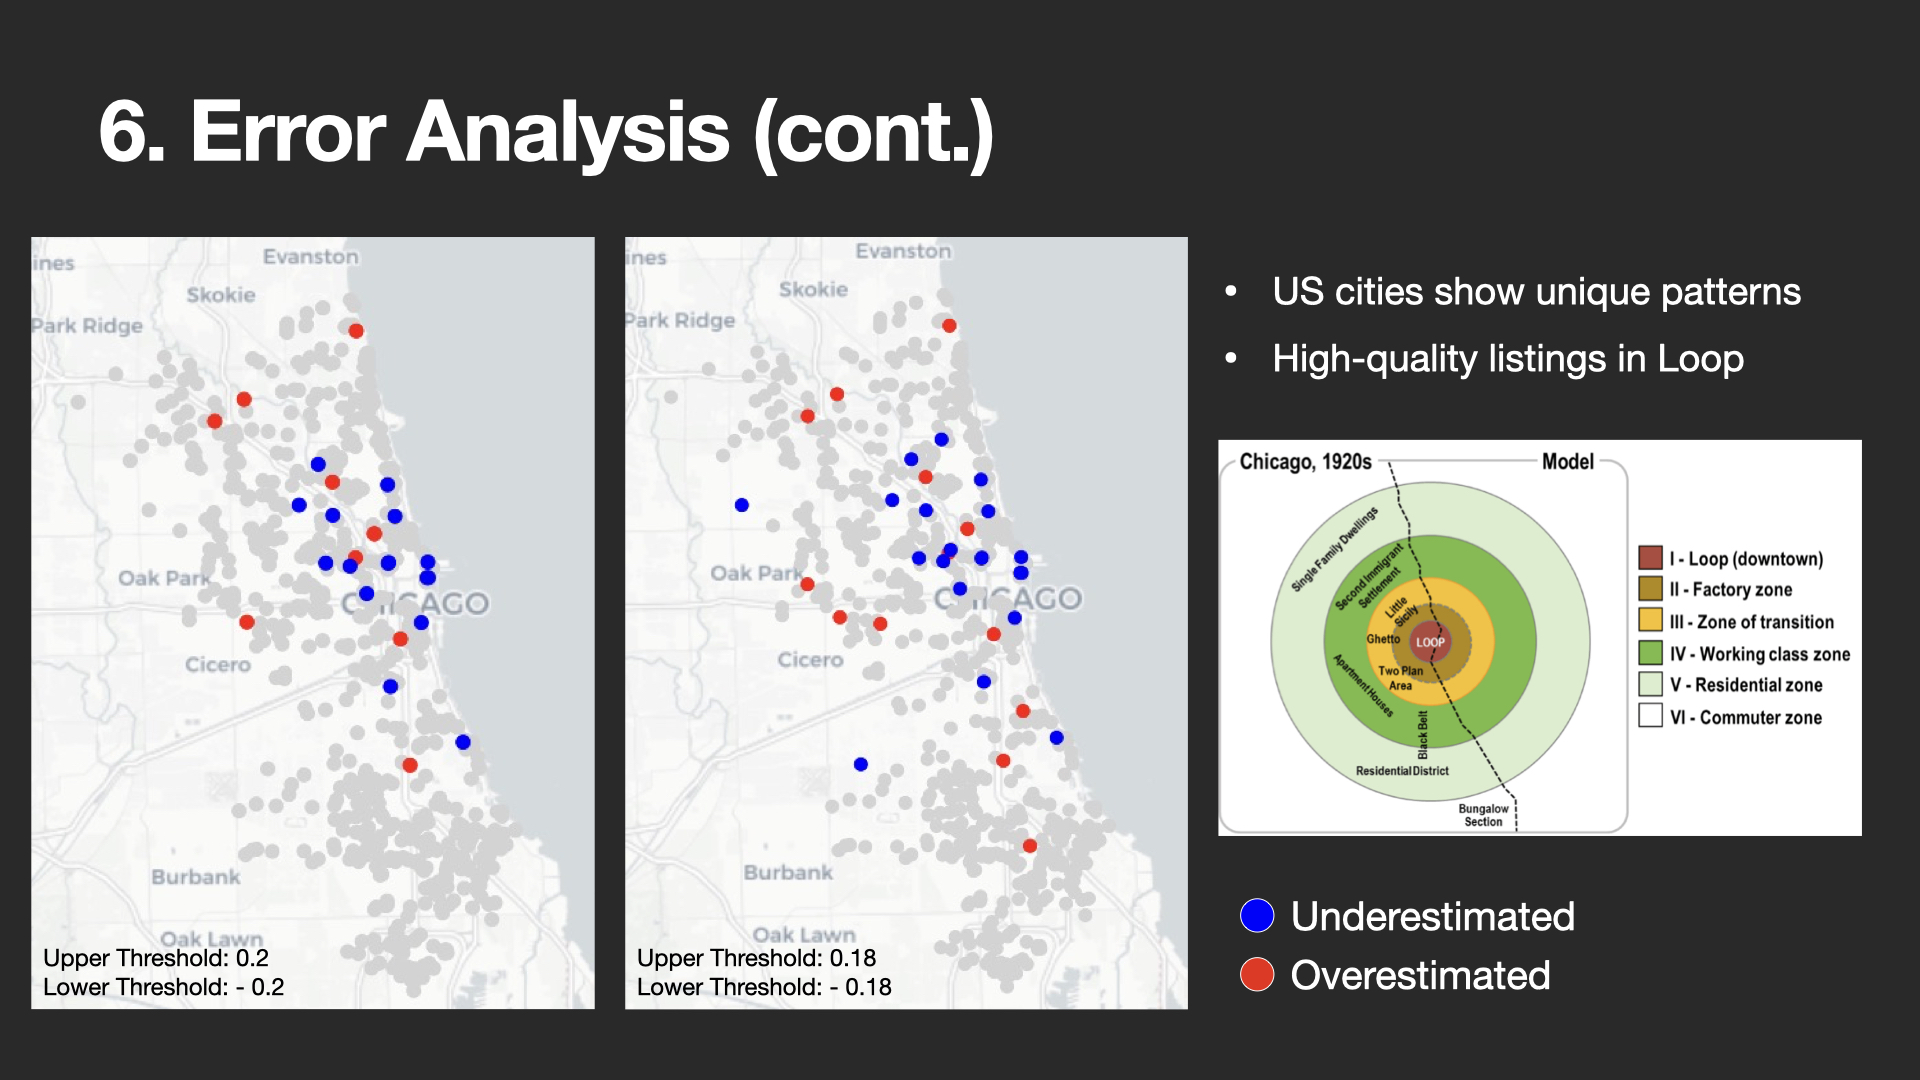
\includegraphics[width=\textwidth]{Visual/examplemap.jpeg}
  \caption{Example Map}
\end{figure}

\end{document}


% You can make this a bit easier if you use the subfile package
